% This is samplepaper.tex, a sample chapter demonstrating the
% LLNCS macro package for Springer Computer Science proceedings;
% Version 2.21 of 2022/01/12
%
\documentclass[runningheads]{llncs}
%
\usepackage[T1]{fontenc}
% T1 fonts will be used to generate the final print and online PDFs,
% so please use T1 fonts in your manuscript whenever possible.
% Other font encondings may result in incorrect characters.
%
\usepackage{graphicx}
% Used for displaying a sample figure. If possible, figure files should
% be included in EPS format.
%
% If you use the hyperref package, please uncomment the following two lines
% to display URLs in blue roman font according to Springer's eBook style:
%\usepackage{color}
%\renewcommand\UrlFont{\color{blue}\rmfamily}
%\urlstyle{rm}
%
\usepackage{subcaption}
\usepackage{hyperref}
\usepackage{xcolor}
\hypersetup{
    colorlinks=true,
    linkcolor=blue,
    filecolor=magenta,
    urlcolor=blue,
    pdftitle={TheoremView: A Framework for Extracting Theorem-like Environments from Raw PDFs},
    pdfpagemode=FullScreen,
}

\begin{document}
%
\title{TheoremView: A Framework for Extracting Theorem-like Environments from Raw PDFs}
%
%\titlerunning{Abbreviated paper title}
% If the paper title is too long for the running head, you can set
% an abbreviated paper title here
%
\author{Shrey Mishra\inst{1}\orcidID{0009-0004-2357-9593} \and
Neil Sharma\inst{2}\orcidID{0009-0004-2357-9593} \and
Antoine Gauquier\inst{1}\orcidID{0009-0005-9573-6364} \and
Pierre Senellart\inst{1,3}\orcidID{0000-0002-7909-5369}}

\authorrunning{S. Mishra et al.}
% First names are abbreviated in the running head.
% If there are more than two authors, 'et al.' is used.

\institute{DI ENS, ENS, CNRS, PSL University, Inria, Paris, France \\
\email{shrey.mishra@ens.psl.eu, antoine.gauquier@ens.psl.eu, pierre@senellart.com}
\and
Malaviya National Institute of Technology \\
\email{neil.sharma3000@gmail.com}
\and
Institut Universitaire de France (IUF)
}

\maketitle              % typeset the header of the contribution
%
\begin{abstract}
This paper presents TheoremView, a novel framework for extracting proofs and theorems from raw PDF scientific papers without requiring \LaTeX~source files. Our approach combines three modalities (\textbf{font}, \textbf{text}, and \textbf{vision}) with sequential modeling to capture long-term dependencies and layout information. By eliminating OCR preprocessing, TheoremView reduces computational overhead for real-time applications while providing robust automated theorem extraction. Our framework is publicly available at \url{https://gitlab.di.ens.fr/mishra/sys-demo}, with a demonstration video at \url{https://youtu.be/demo-link}.


\keywords{Theorem extraction \and Multimodal learning \and Document analysis \and Machine learning \and Natural language processing}
\end{abstract}


\section{Introduction}
\subsection{Motivation for Theorem Extraction}
In contemporary scientific research, articles are primarily published as PDFs, and many 
search engines index entire papers instead of specific scientific results. This paper 
contributes to TheoremKB ~\cite{doceng_paper}, a project focused on building a knowledge base of mathematical 
results across different fields of science. The objective is to improve the accessibility of 
relevant information for researchers, allowing for more effective retrieval and utilization 
of scientific knowledge. TheoremKB offers several key advantages:
\begin{itemize}
    \item \textbf{Enhanced Accessibility:} Streamlines the retrieval of specific proofs and theorems, allowing quick access to targeted mathematical results compared to traditional full-text search engines
    
    \item \textbf{Facilitated Knowledge Discovery:} Helps researchers uncover connections between disparate mathematical results and their applications, such as exploring NP-hardness in relation to the vertex cover problem
    
    \item \textbf{Identification of Theorem Interdependencies:} Determines which theorems are used in the proofs of others, essential for assessing the impact of errors in foundational results
    
    \item \textbf{Support for Automated Reasoning:} Provides a foundation for developing AI systems
\end{itemize}

\subsection{Prior work on Theorems and Proofs Extraction}

Previous attempts to address this task include the work presented in~\cite{doceng_paper}, which focused on 
initial explorations of extraction from PDFs framed as object detection and text classification problems. 
This approach utilized font visuals and text modalities but operated only at the text-line level. Subsequent 
research, such as~\cite{mishra2024modularmultimodalmachinelearning}, refined the methodology by incorporating contextual information 
surrounding paragraphs and employing multimodal systems to unify the extraction model.
The TheoremView framework offers a user interface to visualize the results extracted by various models in 
an end-to-end system that directly takes PDFs as input and displays the extracted results. It is designed 
modularly, allowing users to select which model to utilize for extraction, thereby leveraging different 
modalities that highlight the strengths and weaknesses of each approach. This flexibility enables users 
to run models on low-compute hardware, such as systems without GPU instances, for inference. The primary 
objective of this paper is to present an easy-to-use interface that facilitates preprocessing and inference 
in a modular manner.

\section{Methodology}
We propose a modular approach to extract raw information from PDFs. We utilize \textbf{Grobid}~\cite{GROBID} and \textbf{pdfalto}~\cite{pdfalto} to convert 
the documents into valid XML formats. The XML generated by Grobid organizes the content into paragraphs, 
while the XML from pdfalto provides details segmented into text lines along with associated font information. 
We then employ a merging script to correlate the font information with each paragraph extracted by Grobid. 
This process yields a CSV file structured by paragraphs, where each row includes the spatial location of the 
paragraph on the page (indicating the page number as well as vertical and horizontal coordinates), the textual content 
extracted from Grobid, and the font information used within those paragraphs. For a schematic diagram on data pipeline
refer to Figure \ref{fig:datapipeline}.

\begin{figure}[h]
    \centering
    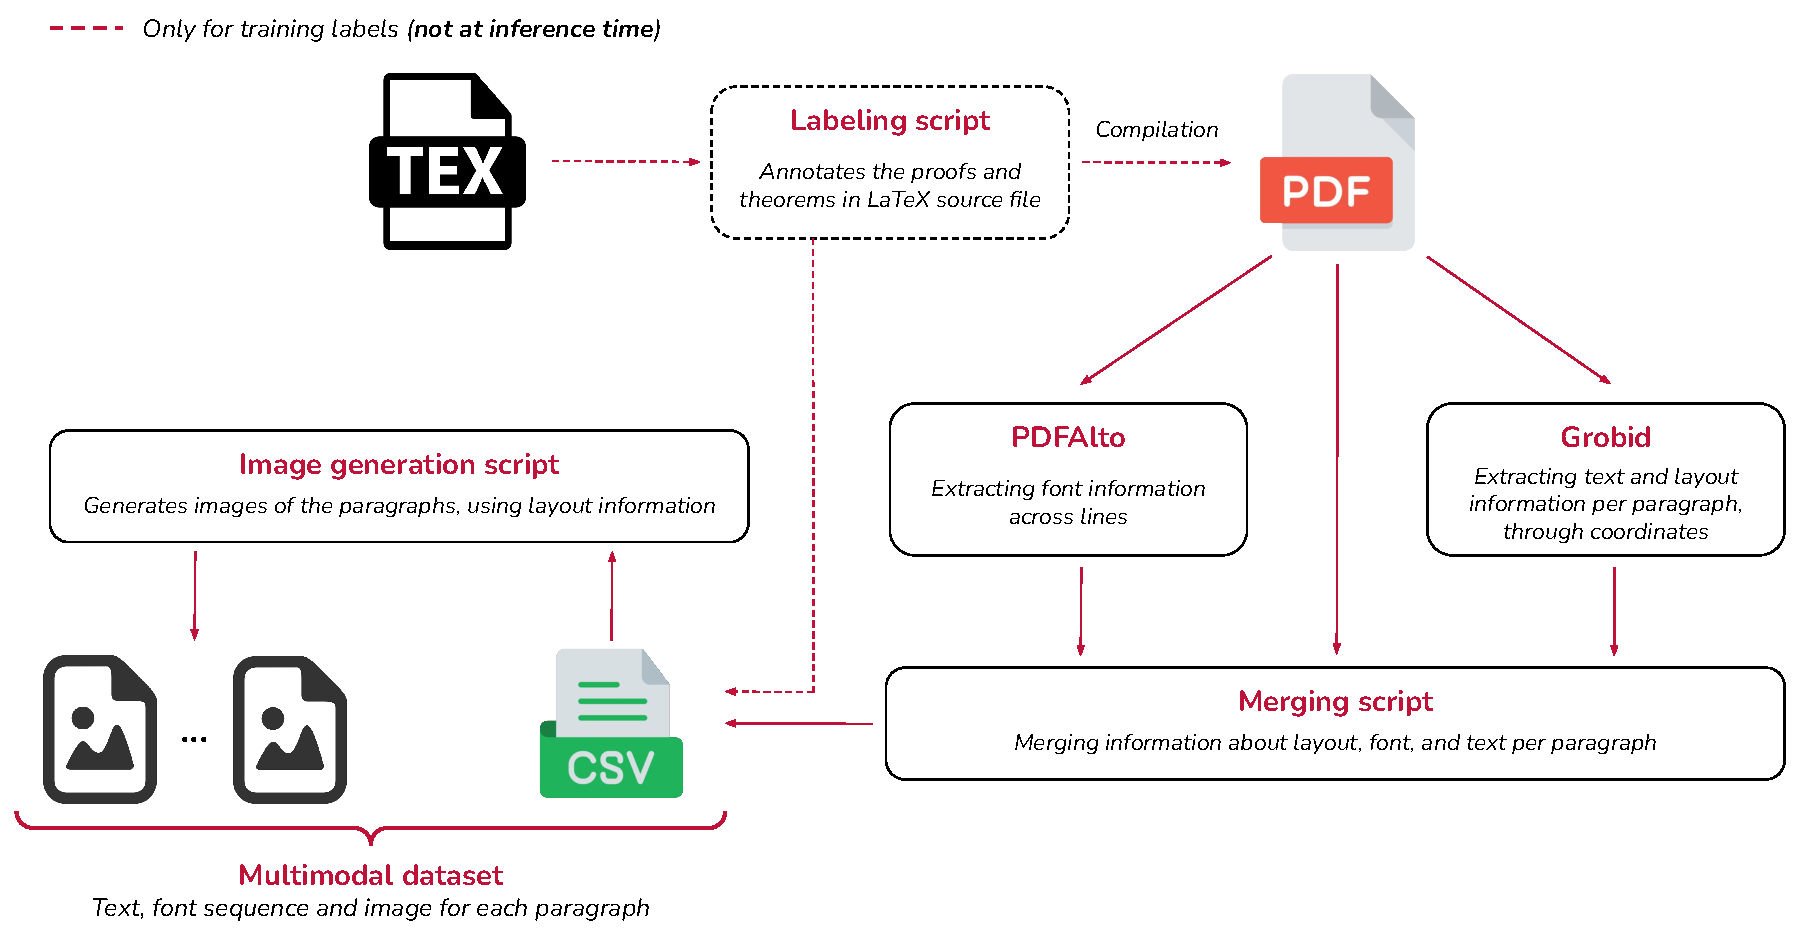
\includegraphics[width=0.65\textwidth]{images/preprocessing.pdf}
    \caption{Data pipeline for extracting and processing information from PDFs.}
    \label{fig:datapipeline}
\end{figure}

Once the information is stored in CSV format, we process the font information using an \textbf{LSTM}~\cite{hochreiter1997long} model, where 
each font is encoded as a unique token to train the network. Simultaneously, we utilize the bitmap image 
rendering of each paragraph to train an \textbf{EfficientNetV2} model \cite{efficientnet}. Additionally, we employ a pretrained from scratch \textbf{RoBERTa} language model \cite{mishra:tel-04665528}, 
on scientific corpus, to make predictions based on the tex modality. Subsequently, we 
integrate all three trained models into a unified multimodal architecture, freezing their weights of each modality backbone and adding 
additional layers to capture intermodality interactions through mechanisms like Gated Multimodal Units 
(GMU)~\cite{arevalo2020gated} or cross-modality attention similar to ViLBERT~\cite{DBLP:conf/nips/LuBPL19} that capture intermodality dependencies. Refer to Figure \ref{fig:generalpipeline} for feature extraction.


\begin{figure}[h]
    \centering
    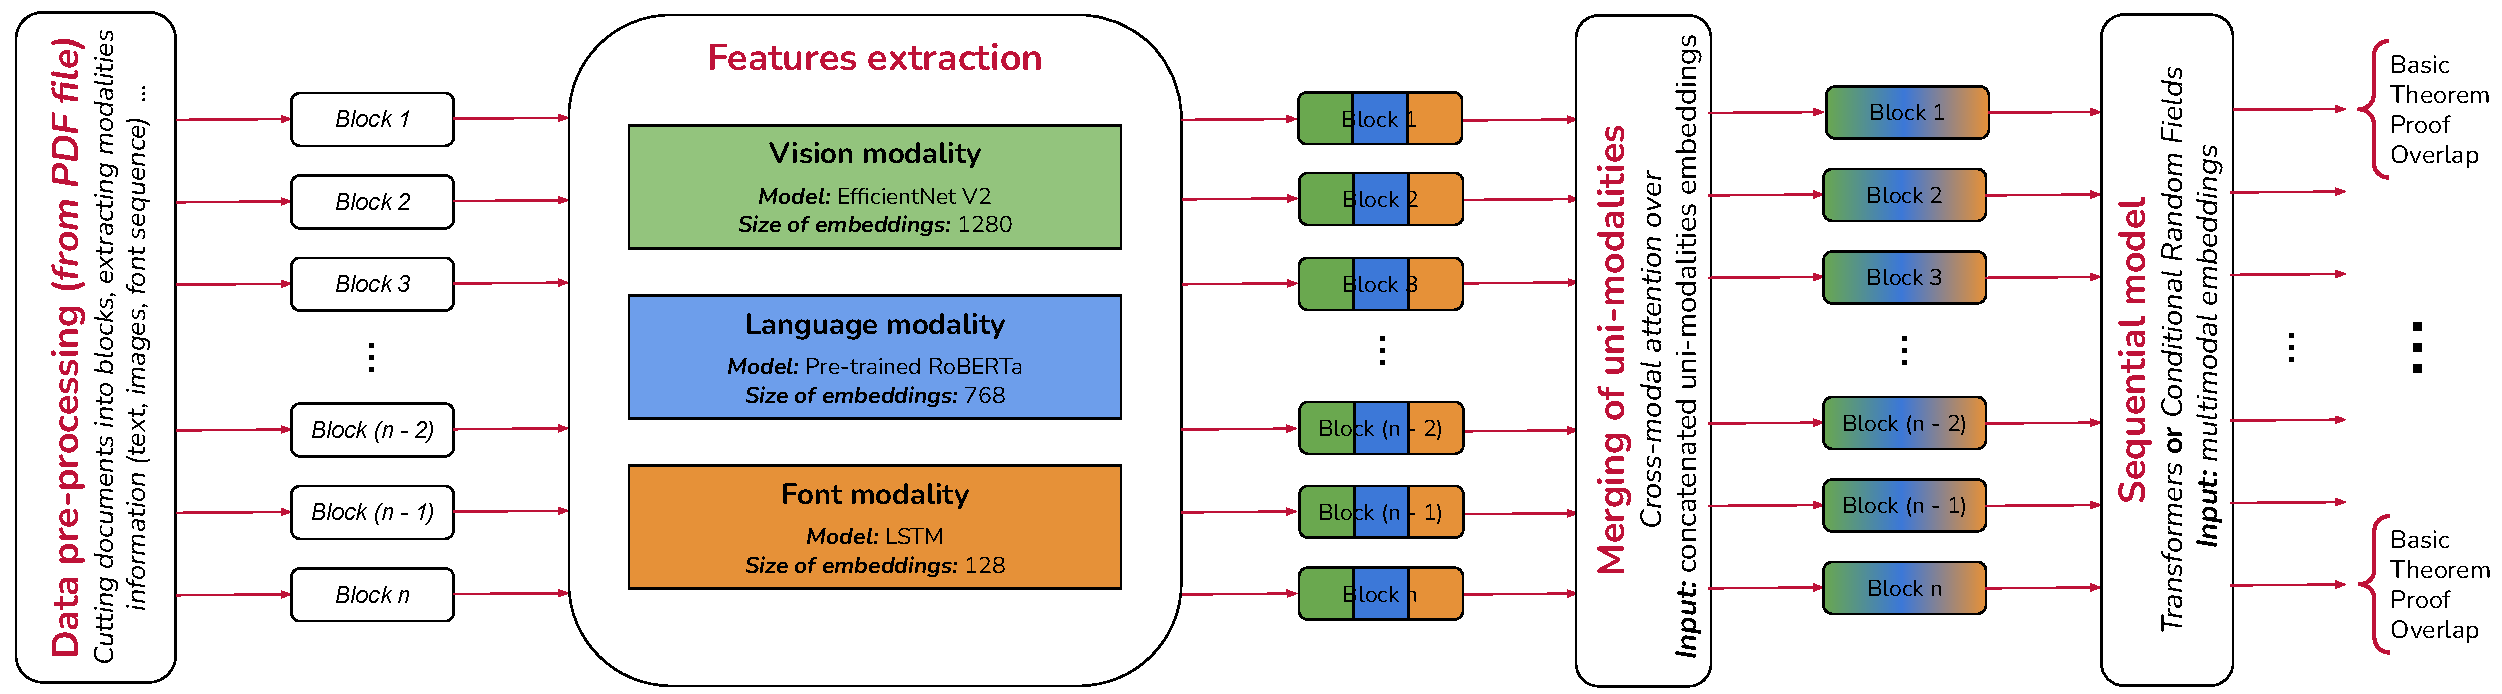
\includegraphics[width=\textwidth]{images/general_pipeline.pdf}
    \caption{Model inference pipeline (adding the sequential paragraph component)}
    \label{fig:generalpipeline}
\end{figure}


With a set of base features extracted from either the unimodal or multimodal approaches, we generate 
features for all paragraphs within the PDF. This process incorporates normalized page information, 
normalized coordinate data for each paragraph, and paragraph embeddings derived from the raw features 
just before the softmax layer. To capture sequential information across multiple paragraphs, we train a 
Conditional Random Field (CRF)~\cite{crf} or Transformer layer on top of the extracted features. The goal is to utilize 
relative information to contextualize each paragraph and accurately determine its label. Our model 
categorizes paragraphs into four major classes: (1) \textbf{Proof-like}, (2) \textbf{Theorem-lik}, (3) \textbf{Basic} (neither 
proof nor theorem), and (4) an \textbf{Overlap} reject class that arises from preprocessing discrepancies.

\section{Demonstation scenario}

The TheoremView demo interface, built using Streamlit, follows a modular architecture with distinct functional components. The frontend allows users to upload PDFs or select from cached samples for metadata processing using Grobid and pdfalto tools, with results stored as CSV files. Users can run various ML models (unimodal or multimodal) through a pipeline that calculates processing time, generates bounding boxes, creates cropped images of theorems/proofs, and produces analytical graphs. The system implements efficient caching using pickle files for frequently accessed PDFs and ML model results.

\begin{figure}[h]
    \centering
    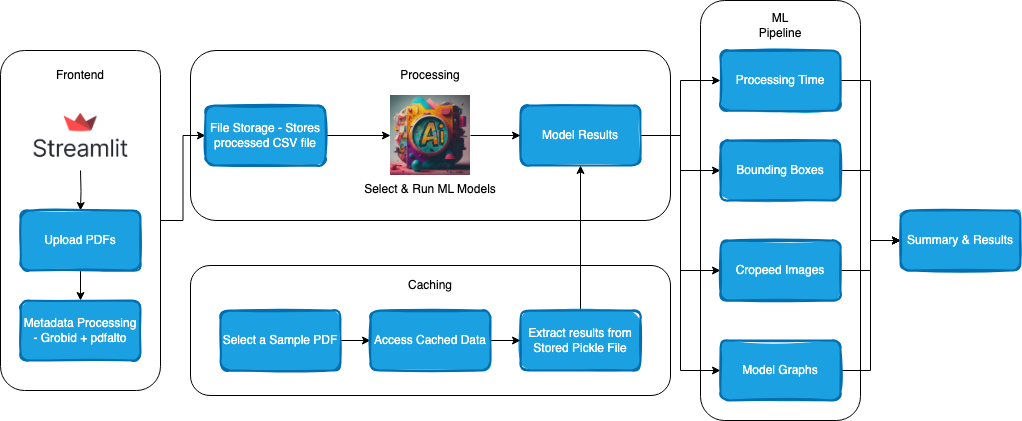
\includegraphics[width=0.75\textwidth]{images/sys-demo-arch.png}
    \caption{Systems architecture of the various UI components
    }
    \label{fig:system-arch}
\end{figure}

The UI of the demo is organized into several segments (for an overview see Figure~\ref{fig:system-arch}), each serving a specific function:

\begin{enumerate}
    \item \textbf{Upload and Process}: Users can upload PDFs or select from cached examples. The system processes PDFs using Grobid and pdfalto, converts pages to bitmap images, and merges XML outputs to generate a preprocessed \texttt{data.csv} file.

    \item \textbf{Predict and Preview}: Users can select unimodal or multimodal base models, with optional sequential processing using CRF, Transformer, or none, offering 12 possible combinations. Results can be previewed or downloaded (see Figure \ref{fig:predictions_and_vis}).

    \item \textbf{Summary and Statistics}: Provides breakdown of inference time for current and cached runs, enabling comparative analysis.
\end{enumerate}



% \begin{figure}[h]
    %     \centering
    %     \begin{subfigure}{0.45\textwidth}
    %         \centering
    %         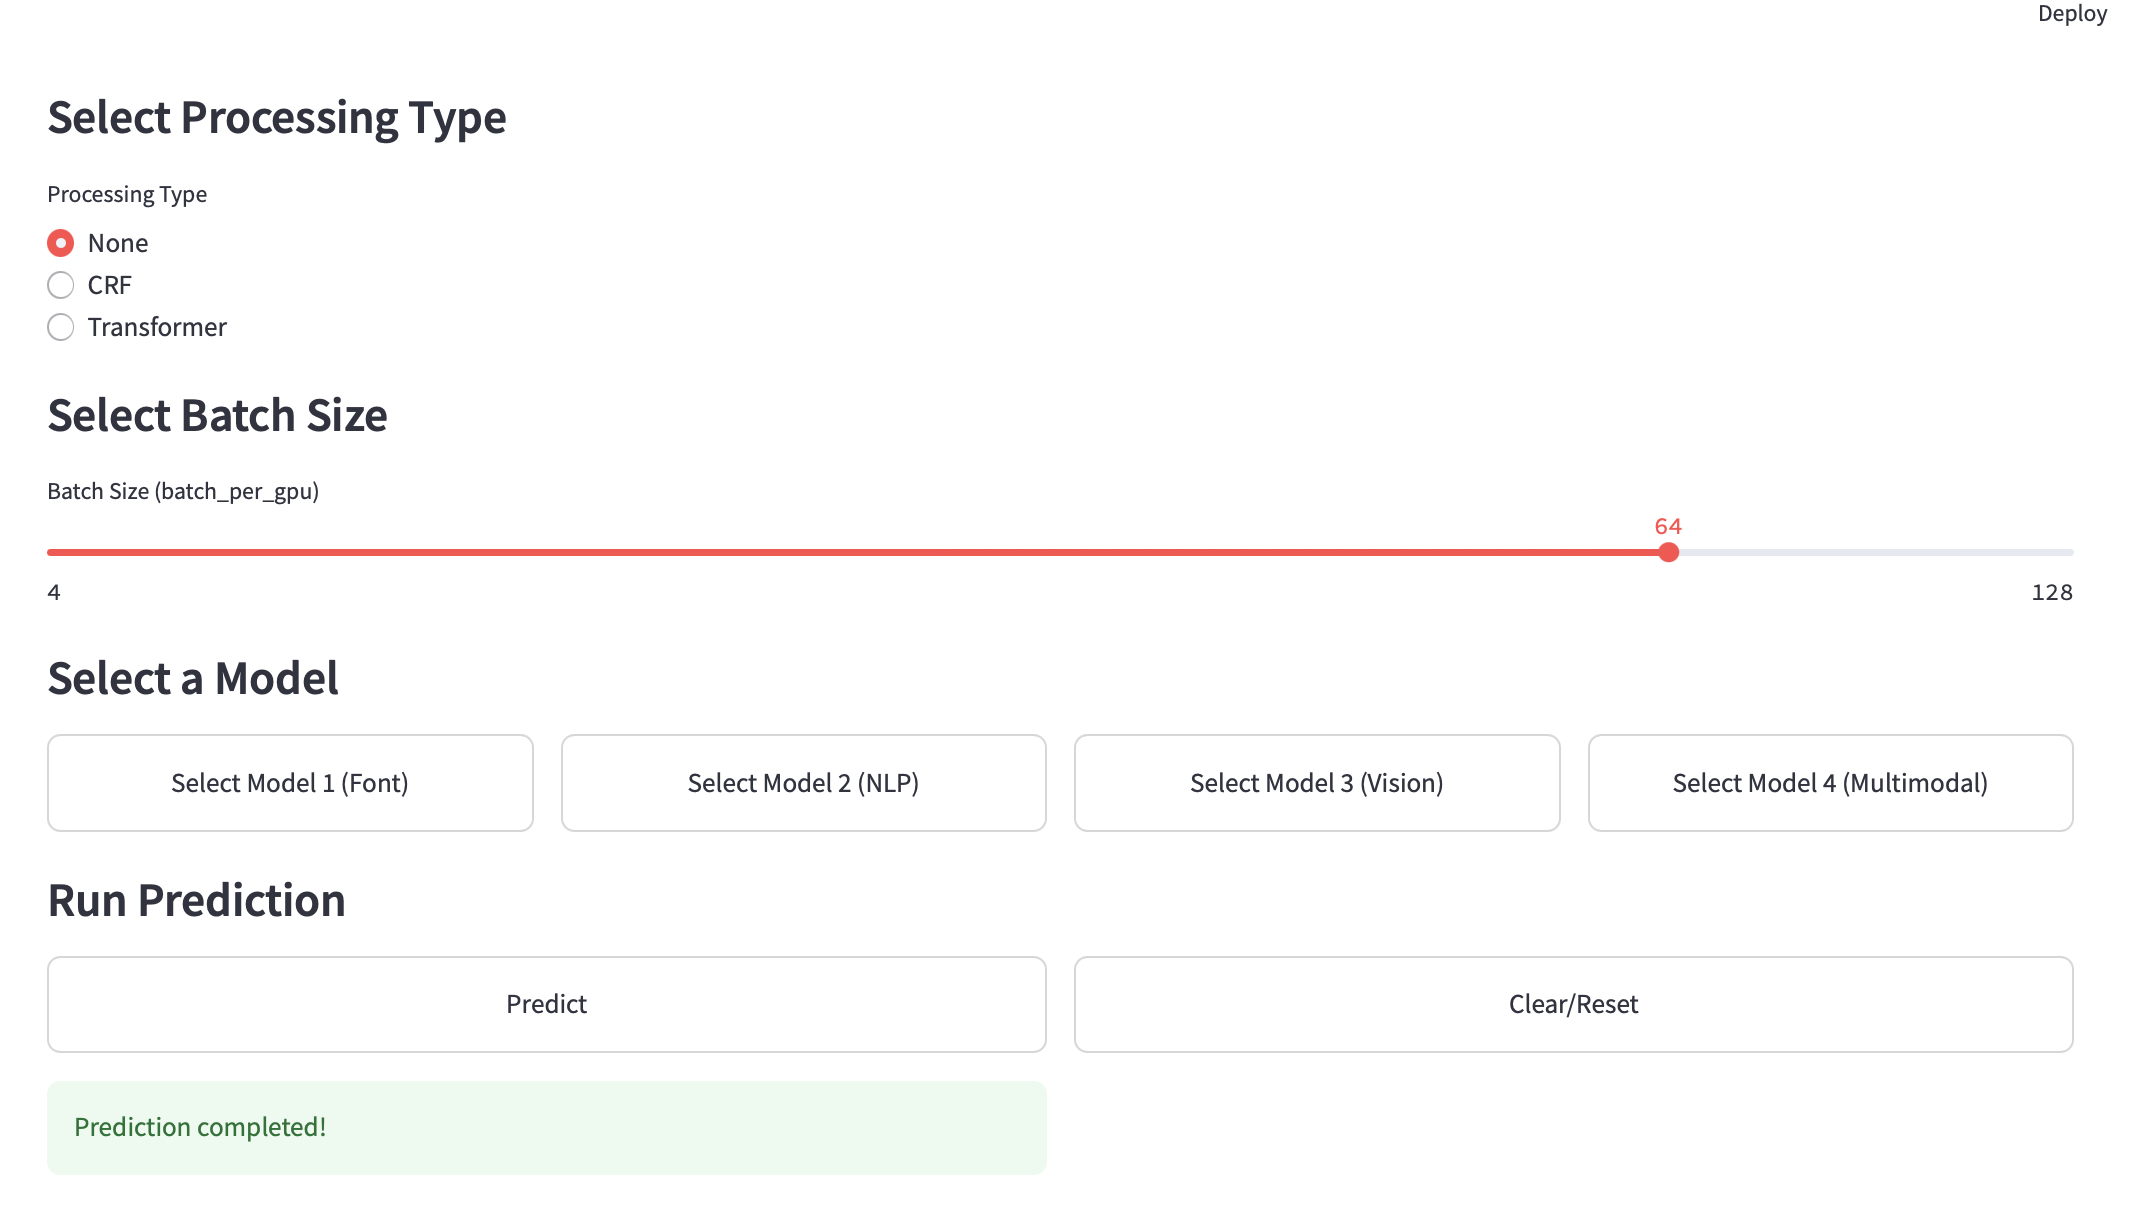
\includegraphics[width=\textwidth]{images/buttons.png}
    %         \caption{UI Buttons to run select the prediction model}
    %         \label{fig:buttons}
    %     \end{subfigure}
    %     \hfill
    %     \begin{subfigure}{0.45\textwidth}
    %         \centering
    %         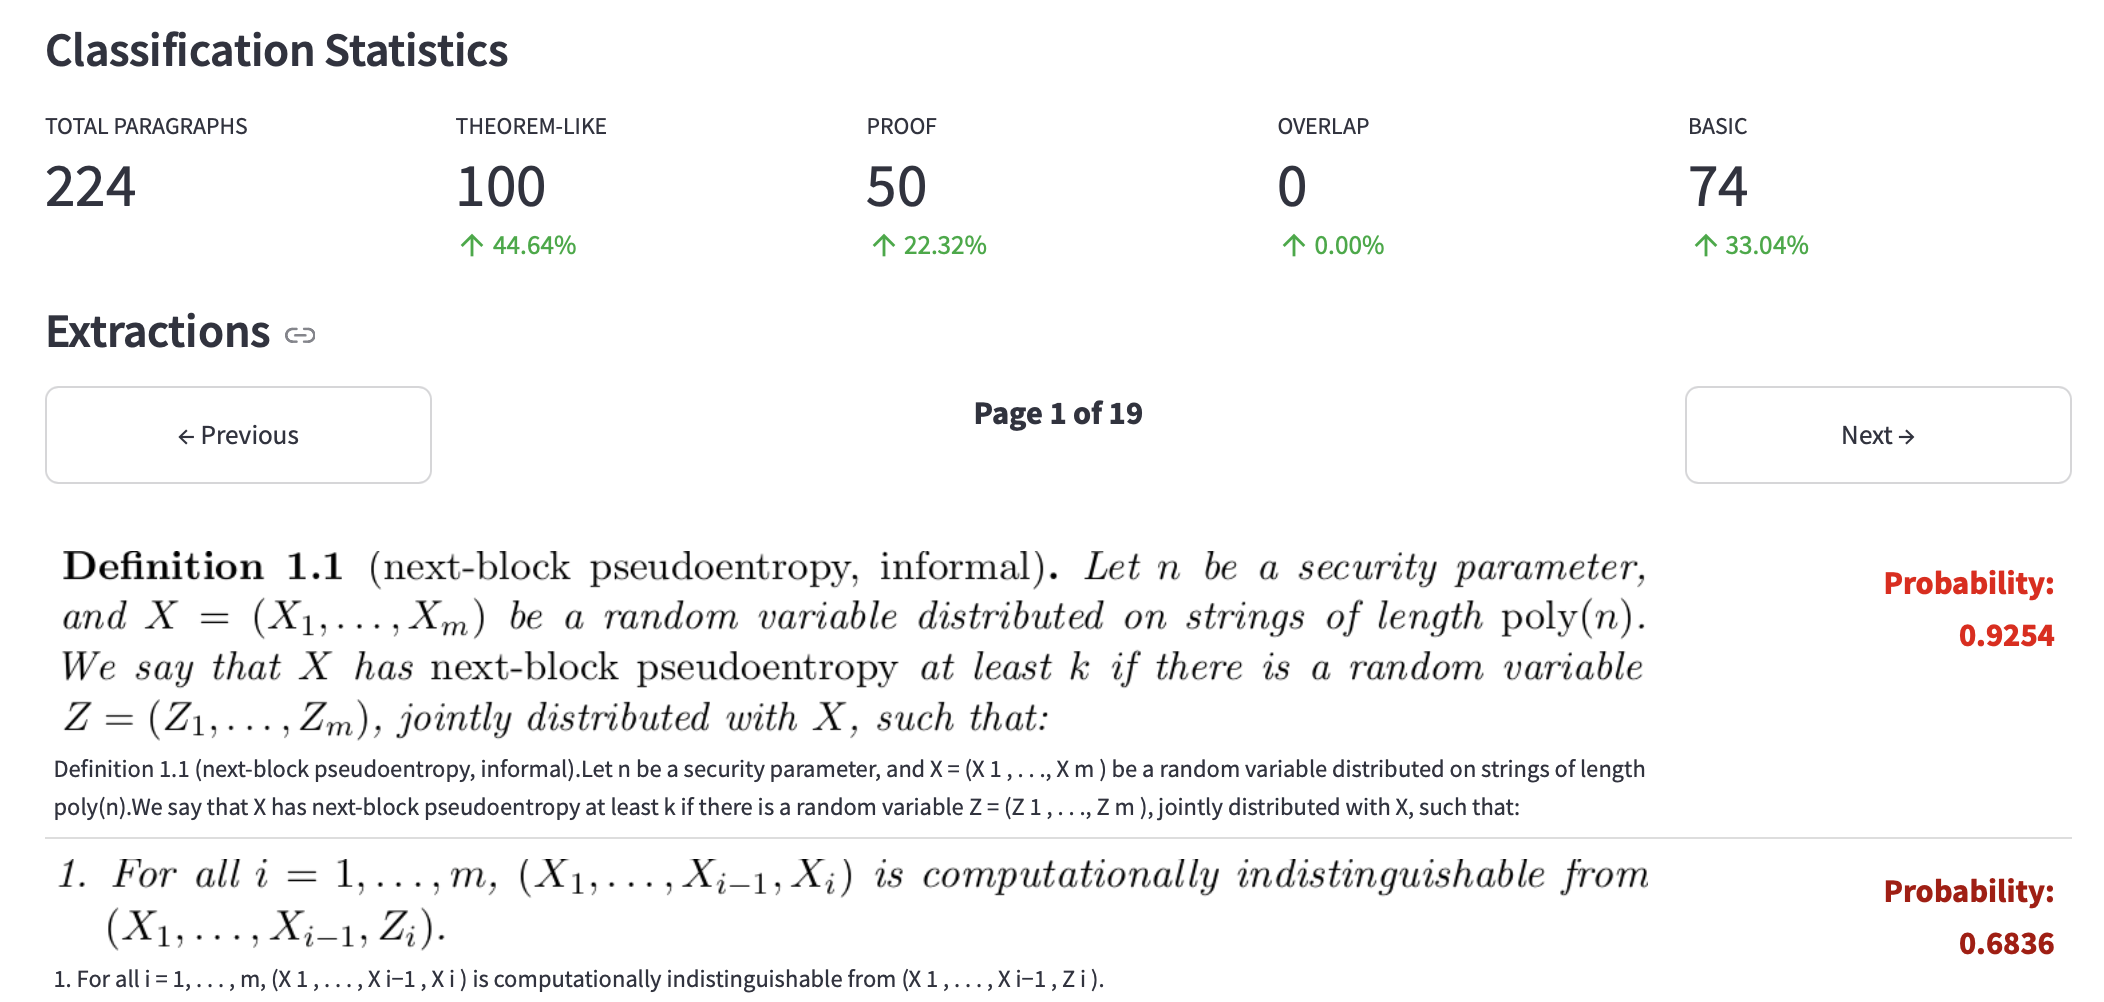
\includegraphics[width=\textwidth]{images/extractions.png}
    %         \caption{Extracted Information}
    %         \label{fig:extractions}
    %     \end{subfigure}
    %     \vskip\baselineskip
    %     \begin{subfigure}{0.45\textwidth}
    %         \centering
    %         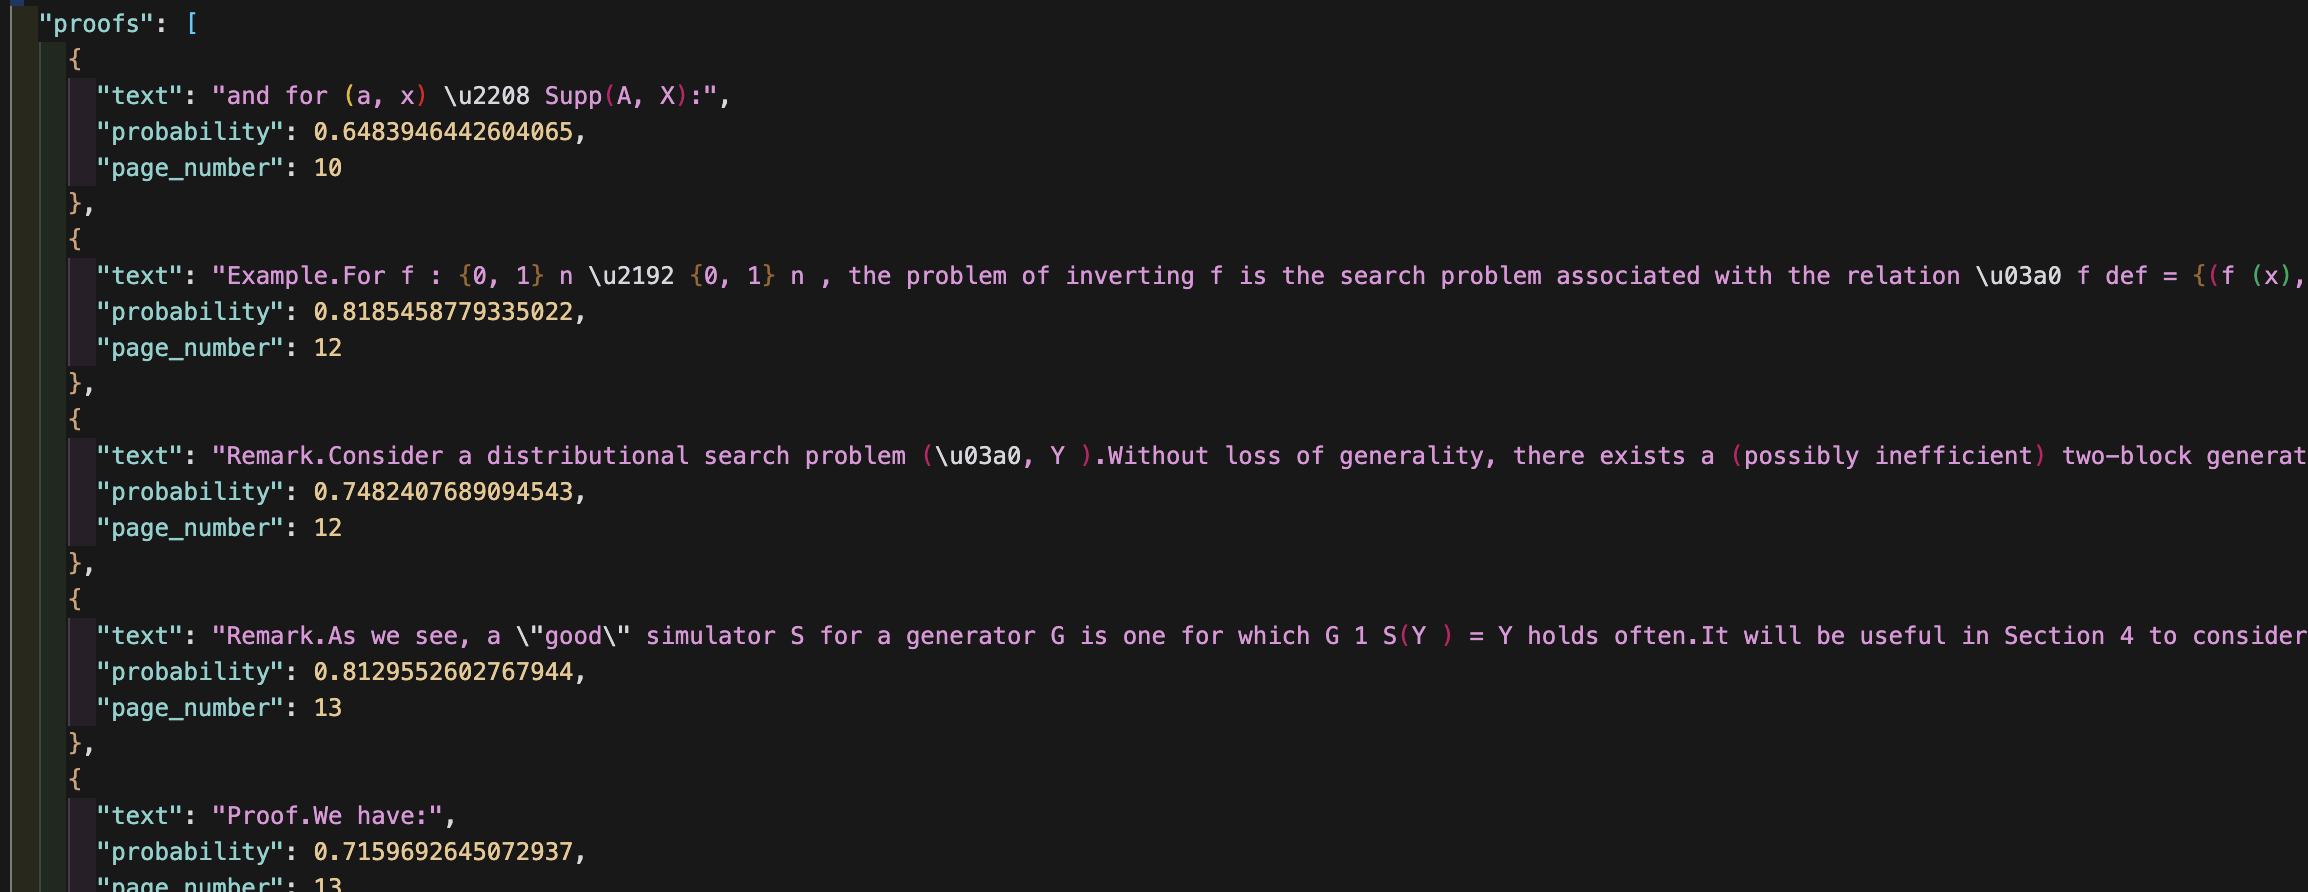
\includegraphics[width=\textwidth]{images/json_output.png}
    %         \caption{Extracted Information in JSON format.}
    %         \label{fig:json_output}
    %     \end{subfigure}
    %     \hfill
    %     \begin{subfigure}{0.45\textwidth}
    %         \centering
    %         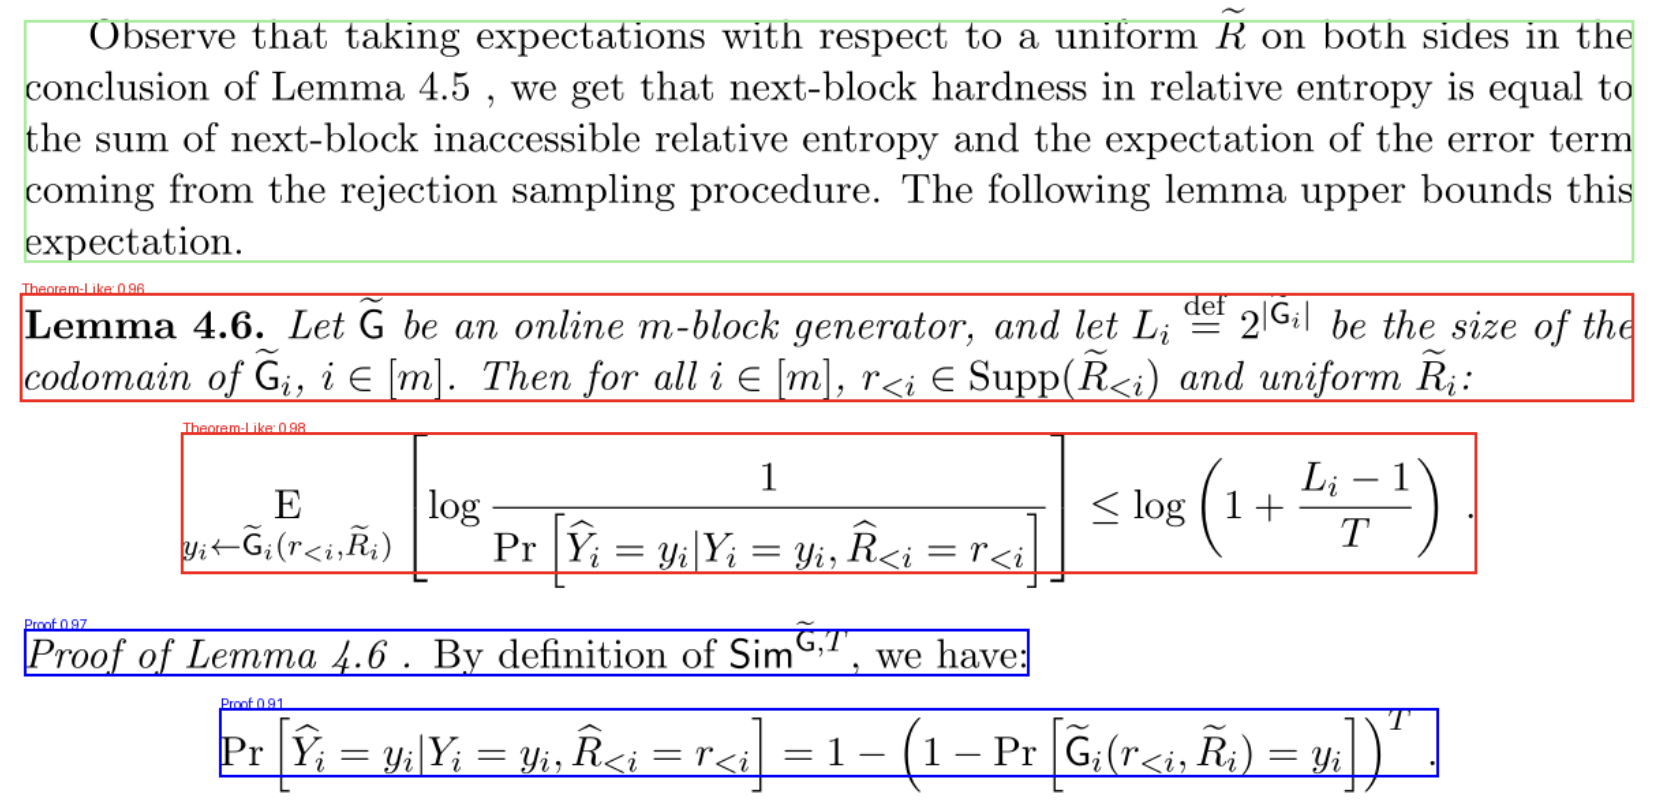
\includegraphics[width=\textwidth]{images/vis_on_pdf.png}
    %         \caption{Visualizations annotated on the PDF.}
    %         \label{fig:vis_on_pdf}
    %     \end{subfigure}
    %     \caption{Various visual elements in the demo.}
    %     \label{fig:combined}
    % \end{figure}

\begin{figure}[h]
    \centering
    \begin{subfigure}[b]{0.6\textwidth}
        \centering
        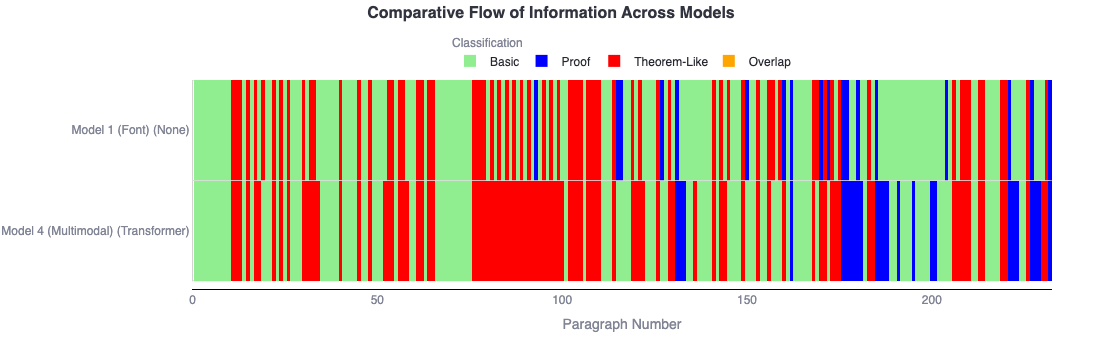
\includegraphics[width=\textwidth]{images/comparitive-v3.png}
        \caption{Flow of information across paragraphs}
        \label{fig:model_comp}
    \end{subfigure}
    \hfill
    \begin{subfigure}[b]{0.35\textwidth}
        \centering
        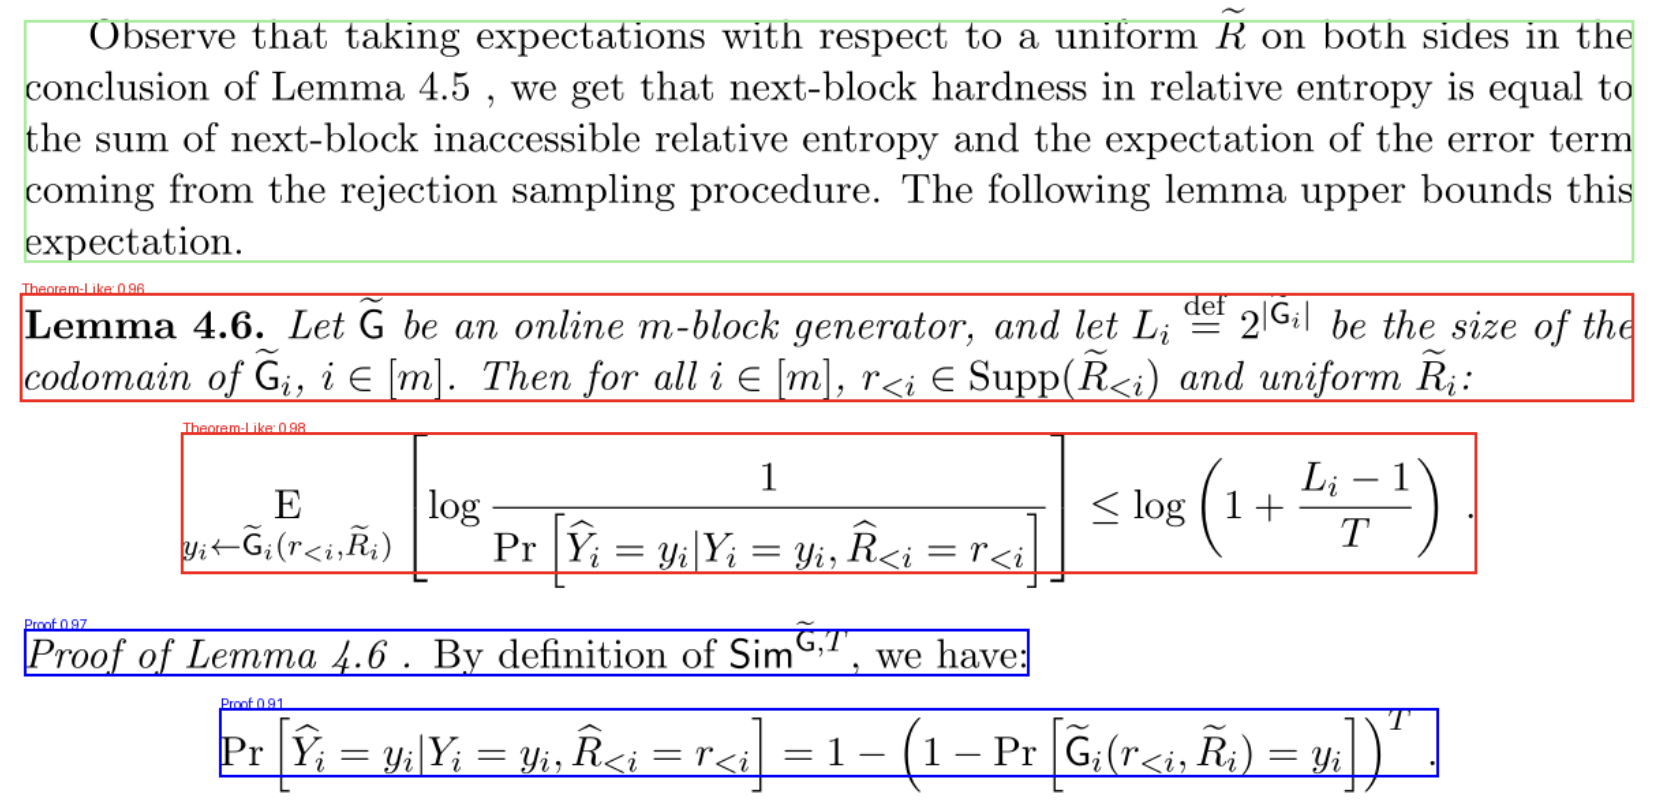
\includegraphics[width=\textwidth]{images/vis_on_pdf.png}
        \caption{Visualization of predictions annotated on the PDF}
        \label{fig:vis_on_pdf}
    \end{subfigure}
    \caption{Visualizing model predictions}
    \label{fig:predictions_and_vis}
\end{figure}

%
\begin{thebibliography}{10}

\bibitem{mishra2024modularmultimodalmachinelearning}
Mishra, S., Gauquier, A., Senellart, P.: Modular Multimodal Machine Learning for Extraction of Theorems and Proofs in Long Scientific Documents (Extended Version). arXiv preprint arXiv:2307.09047 (2024). \url{https://arxiv.org/abs/2307.09047}

\bibitem{mishra:tel-04665528}
Mishra, S.: Multimodal Extraction of Proofs and Theorems from the Scientific Literature. PhD thesis, Universit{\'e} Paris Sciences \& Lettres (2024). \url{https://hal.science/tel-04665528}


\bibitem{doceng_paper}
Mishra, S., Pluvinage, L., Senellart, P.: Towards extraction of theorems and proofs in scholarly articles. In: Healy, P., Bilauca, M., Bonnici, A. (eds.) DocEng '21: ACM Symposium on Document Engineering 2021, Limerick, Ireland, August 24-27, 2021, pp. 25:1--25:4. Association for Computing Machinery, New York, NY, USA (2021). \doi{10.1145/3469096.3475059}

\bibitem{mishra2024first}
Mishra, S., Brihmouche, Y., Delemazure, T., Gauquier, A., Senellart, P.: First steps in building a knowledge base of mathematical results. In: Proceedings of the Fourth Workshop on Scholarly Document Processing (SDP 2024), pp. 165--174 (2024)

\bibitem{hochreiter1997long}
Hochreiter, S., Schmidhuber, J.:  Long short-term memory. In: Neural Computation 9, 8 (1997)

\bibitem{arevalo2020gated}
Arevalo, J., Solorio, T., Montes-y Gómez, M., A González, F.: Gated multimodal networks. In: Neural Computing and Applications 32 (2020). 

\bibitem{GROBID}
GROBID: \url{https://github.com/kermitt2/grobid}, GitHub (2008--2024). swh:1:dir:dab86b296e3c3216e2241968f0d63b68e8209d3c

\bibitem{pdfalto}
pdfalto: \url{https://github.com/kermitt2/pdfalto}, GitHub (2017--2024). swh:1:dir:4b5e8b8c8e3c3216e2241968f0d63b68e8209d3c

\bibitem{efficientnet}
Tan, M., Le, Q.V.: EfficientNetV2: Smaller Models and Faster Training. In: Proceedings of the 38th International Conference on Machine Learning, PMLR 139, pp. 10096--10106 (2021)

\bibitem{crf}
Lafferty, J., McCallum, A., Pereira, F.C.N.: Conditional Random Fields: Probabilistic Models for Segmenting and Labeling Sequence Data. In: Proceedings of the Eighteenth International Conference on Machine Learning, ICML '01, pp. 282--289. Morgan Kaufmann Publishers Inc., San Francisco, CA, USA (2001)

\bibitem{transformer}
Vaswani, A., Shazeer, N., Parmar, N., Uszkoreit, J., Jones, L., Gomez, A.N., Kaiser, Ł., Polosukhin, I.: Attention is All you Need. In: Advances in Neural Information Processing Systems, pp. 5998--6008 (2017)

\bibitem{DBLP:conf/nips/LuBPL19}
Lu, J., Batra, D., Parikh, D., Lee, S.: ViLBERT: Pretraining Task-Agnostic Visiolinguistic Representations for Vision-and-Language Tasks. In: Advances in Neural Information Processing Systems 32: Annual Conference on Neural Information Processing Systems 2019, NeurIPS 2019, Vancouver, BC, Canada, pp. 13--23 (2019)

\end{thebibliography}
\end{document}
